\documentclass[12pt, a4paper]{article}
\title{Изучение дифракции света (4.3.1)}
\author{Стеценко Георгий, Б02-312}
\date{}
% !TeX encoding = UTF-8

\usepackage{geometry}
\usepackage{amsmath, amsfonts, amssymb, amsthm} % стандартный набор AMS-пакетов для математ. текстов
\usepackage{mathtext}
\usepackage[utf8]{inputenc} % кодировка utf8
\usepackage[russian]{babel} % русский язык
\usepackage[pdftex,dvipsnames]{xcolor} % работа с цветами
\usepackage[pdftex]{graphicx} % графика (картинки)
\usepackage{tikz,pgfplots} % рисунки
\usepackage{indentfirst}
%\usepackage[labelfont=bf,labelsep=endash,skip=3pt]{caption} % подпись картинок
% \usepackage{fancyhdr,pageslts} % настройка колонтитулов
\usepackage{enumitem} % работа со списками
\usepackage{floatrow,multicol,multirow,longtable,hhline} % работа с таблицами
\usepackage{float,wrapfig} % плавающие объекты
\usepackage{tcolorbox} % рамка вокруг текста
%\usepackage[calc]{datetime2} % дата
\usepackage{bm} % жирное начертание в формулах
\usepackage{physics} % физический пакет
\DeclareMathAlphabet\mathbfcal{OMS}{cmsy}{b}{n}
\usepackage{pgfornament} % красивые рюшечки и вензеля
\usepackage{mdframed}
\usepackage{derivative}
\usepackage{mathrsfs} %EDS
\usepackage{soul} % strikethorugh
%\usepackage{boondox-cal}

% ----------------------------------------
% Настройка шрифта

% Просто закооментируйте следующую строчку, если не работает. Будет другой шрифт, правда :(
% \usepackage{pscyr}

% ----------------------------------------
% Стилевые настройки

\usepackage{boldline} % жирная линия после таблиц (чтобы не было ошибок, этот пакет должен подключаться именно тут!)
\floatsetup[table]{style=Plaintop,floatrowsep=qquad} % настройка оформления таблиц
\setlist[enumerate,itemize]{leftmargin=5mm,itemindent=10mm,itemsep=0mm,
listparindent=0em,labelsep=2mm,topsep=2mm,labelwidth=4mm} % настройки списков

\setlength{\columnsep}{0.5cm} % расстояние между колонками
\setlength{\parskip}{1pt} % расстояние до текста от колонтитула

%\usepackage{titlesec} % управление оформлением section
%\renewcommand{\thesection}{\Roman{section}}
%\titleformat{\section}[block]{\bfseries\large}{\thesection.}{5pt}{}

% ----------------------------------------
% Настройки полей
\geometry{
  left=10mm,
  top=10mm,
  right=10mm,
  bottom=15mm,
  marginparsep=0mm,
  marginparwidth=0mm,
  headheight=0pt,
  headsep=0pt,
footskip=20pt}

% ----------------------------------------
% Настройки колонтитулов и нумерации страниц
\pagenumbering{arabic}



\newcounter{ntask}
\setcounter{ntask}{0}


\newcommand{\arsh}{\mathrm{arsh} \,\,}
\newcommand{\arch}{\mathrm{arch} \,\,}
\newcommand{\arth}{\mathrm{arth} \,\,}
\newcommand{\arcth}{\mathrm{arcth} \,\,}
\renewcommand{\Re}{\operatorname{Re} \,}
\newcommand{\EDS}{\mathscr{E}}
\newcommand{\diffract}[1]{\frac{\mathrm{d}#1}{\mathrm{d}t}}

\newcommand{\kHz}{~\mathrm{kHz}}
\newcommand{\GHz}{~\mathrm{GHZ}}
\newcommand{\us}{~\mathrm{\mu s}}
\newcommand{\mim}{~\mathrm{mm}}
\addto\captionsrussian{\def\refname{Источники}}

\begin{document}
\maketitle

\section{Аннотация}
\textbf{Цель работы:} исследовать явления дифракции Френеля и Фраунгофера
на щели, изучить влияние дифракции на разрешающую способность оптических
инструментов.

\textbf{Оборудование и материалы:} оптическая скамья, ртутная лампа, монохроматор,
щели с регулируемой шириной, рамка с вертикальной нитью, двойная щель,
микроскоп на поперечных салазках с микрометрическим винтом, зрительная
труба.

\section{Описание работы, установка и теоретические сведения}
\subsection*{А. Дифракция Френеля}
\begin{figure}[h]
  \includegraphics[width=0.7\linewidth]{pics/0.png}
  \centering
  \caption{Схема установки 1.}
  \label{pic:setup-1}
\end{figure}

Схема установки представлена на Рис. \ref{pic:setup-1}.
Щель $S_2$ освещается параллельным пучком монохроматического света с помощью коллиматора,
образованного объективом $O_1$ и щелью $S_1$, находящейся в его фокусе.
Световые лучи освещают щель $S_2$ и испытывают на ней дифракцию.
Дифракционная картина рассматривается с помощью микроскопа М, сфокусированного на
некоторую плоскость наблюдения П.

Распределение интенсивности света в плоскости П рассчитаем с помощью зон Френеля.
При освещении $S_2$ параллельным пучком лучей (плоская зона) зоны Френеля представляют
собой плоскости, параллельные краям щели. Результирующая амплитуда в точке наблюдения
определеяется суперпозицией колебаний от тех зон Френеля, которые не перекрыты створками щели.
Графическое определение результирующей амплитуды производится с помощью векторной
диаграммы -- спирали Корню. Суммарная ширина $m$ зон Френеля $\xi_m$ определяется соотношением:

\begin{equation}
  \xi_m = \sqrt{mz\lambda},
\end{equation}
где $a$ -- расстояние от щели до плоскости П. Вид наблюдаемой картины определяется \textit{числом Френеля} $\Phi$:
$$
  \Phi^2 = \dfrac{D^2}{z\lambda}
$$
-- число зон Френеля, которые укладываются в ширине щели $D$. $p = \frac{1}{\Phi^2}$ называется \textit{волновым параметром}. Дифракционной картины нет, когда П совпадает с плоскостью щели. При малом удалении от щели $\Phi \gg 1$ и картина наблюдается в узкой убласти на границе света и тени у краёв экрана. При последующих удалениях две группы дифракционных полос перемещаются независимо и каждая образует картину дифракции Френеля на экране. Распределение интенсивности может быть найдено с помощью спирали Корню. При дальнейшем увеличении $a$ две системы полос сближаются и накладываются друг на друга, распределение интенсивности определяется числом зон Френеля в полуширине щели. Если их $m$, то будет набюдаться $m-1$ тёмная полоса.

\subsection*{Б. Дифракция Фраунгофера на щели}

\begin{wrapfigure}{r}{0.3\textwidth}
  \vspace{-12mm}
  \begin{center}
    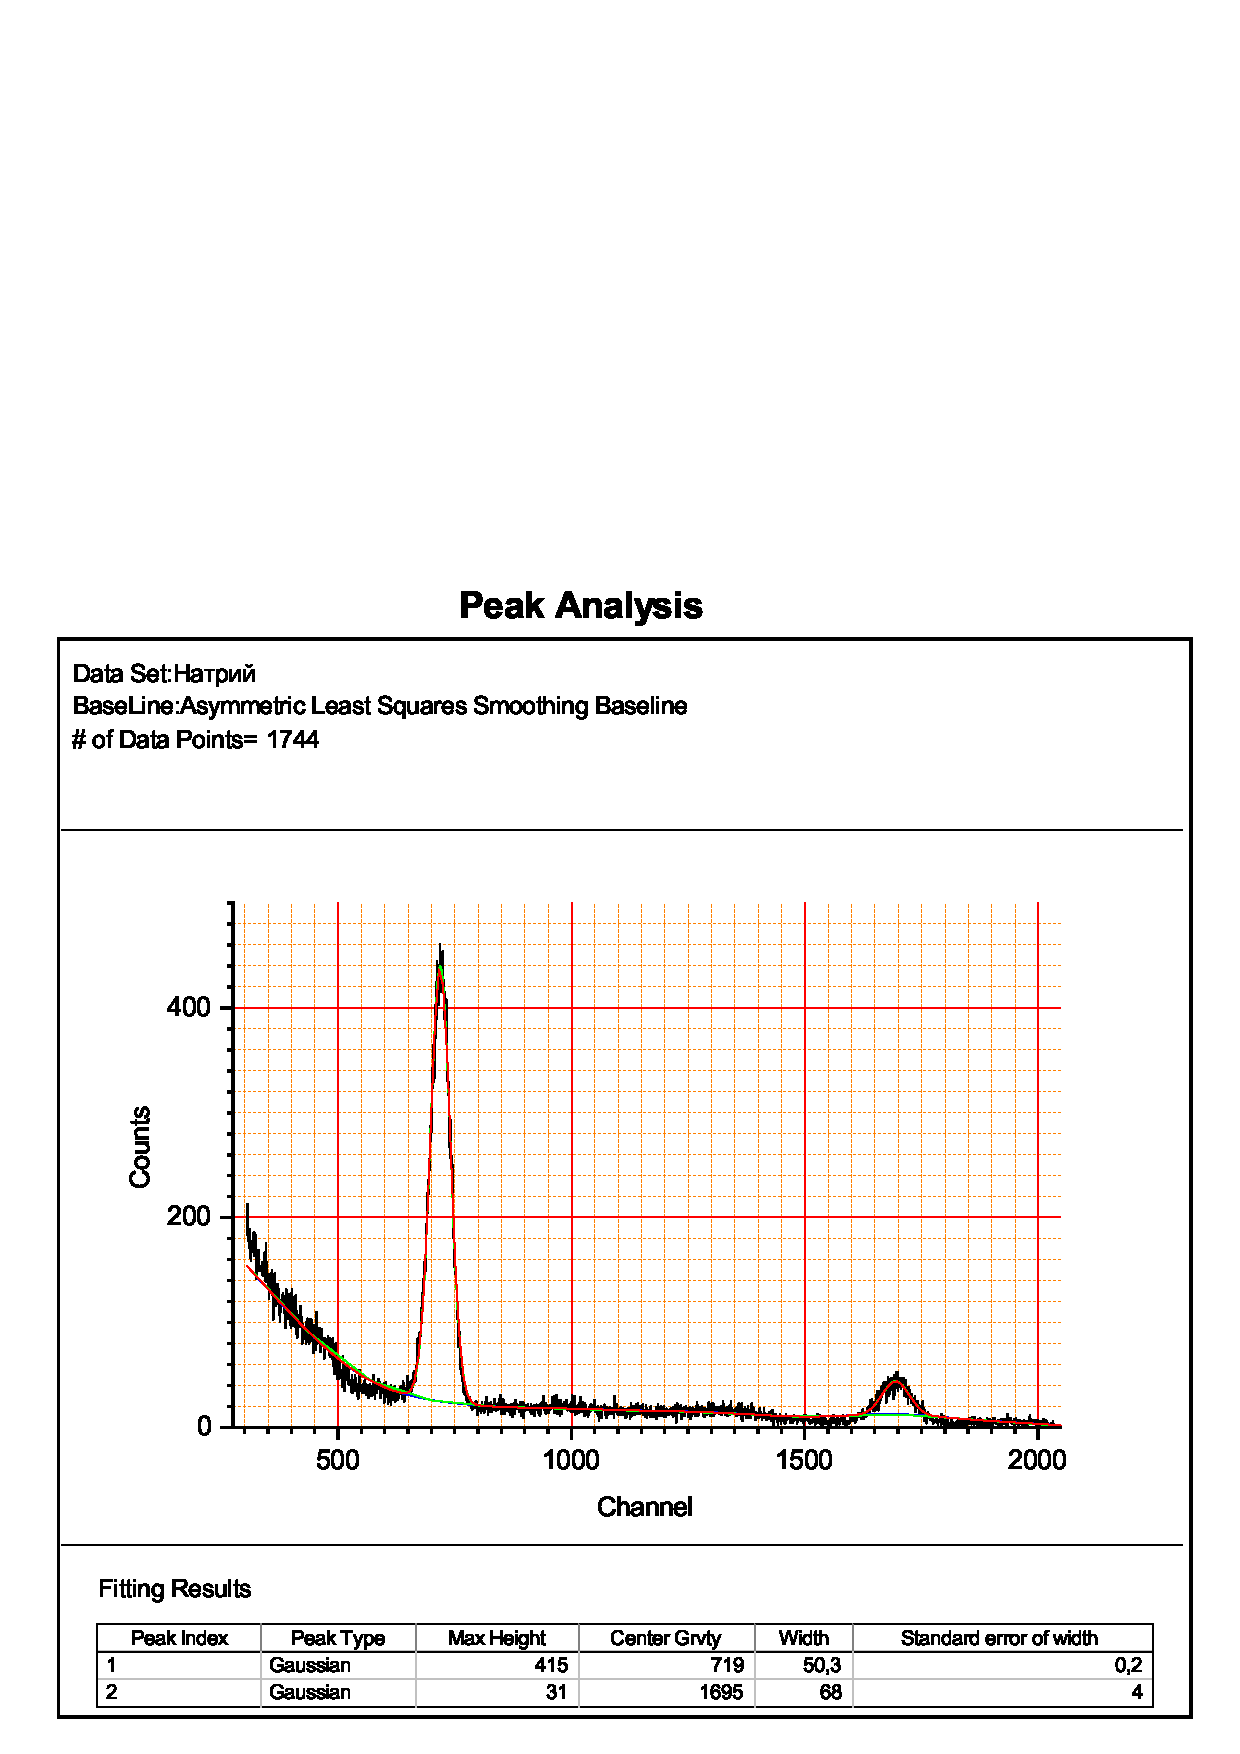
\includegraphics[width = 0.85\linewidth]{pics/1.png}
  \end{center}
  \caption{К фазовым соотношениям при дифракции Фраунгофера}
  \label{pic:fresnel}
\end{wrapfigure}

Рассмотрим действие световой волны действующей из точки $A$ в какой-то точке $B$.
В этом случае можно, взяв точку $M_0$ в качестве центра (см. рис. 1), построить ряд
концентрических сфер, радиусы которых увеличиваются каждый раз на половину
длины волны $\frac{\lambda}{2}$. При пересечении с плоским фронтом волны эти сферы дадут
концентрические окружности. Таким образом, на фронте волны появятся кольцевые зоны (зоны Френеля)
с радиусами $r_1, r_2$ и т. д.

Из геометрических соображений посчитав, можно получить, что
\begin{equation}
  r_m = m \sqrt{a \lambda}
\end{equation}

Картина дифракции упрощается, когда ширина щели становится значительно меньше ширины первой зоны Френеля, т.е. если
\begin{equation}
  D \ll\sqrt{a \lambda}
\end{equation}
Это условие всегда выполняется при достаточно большом $a$. В этом случае дифракционную картину
называют \textit{дифракцией Фраунгофера}. При выполнении пункта $(2)$ у нас упрощаются фазовые
соотношения, что поясняет рис. 2, в итоге с хорошим приближением можно считать, что разность
хода между крайними лучами, приходящими от щели в точке наблюдения $P$, с хорошим приближением равна
\begin{equation}
  \Delta = r_2 - r_1 \approx D \sin \theta \approx D \cdot \theta
\end{equation}
Здесь предполагается, что $\theta$ достаточно мал.
Дифракцию Фраунгофера можно наблюдать на установке с рис. \ref{pic:setup-2}.

\begin{figure}[h]
  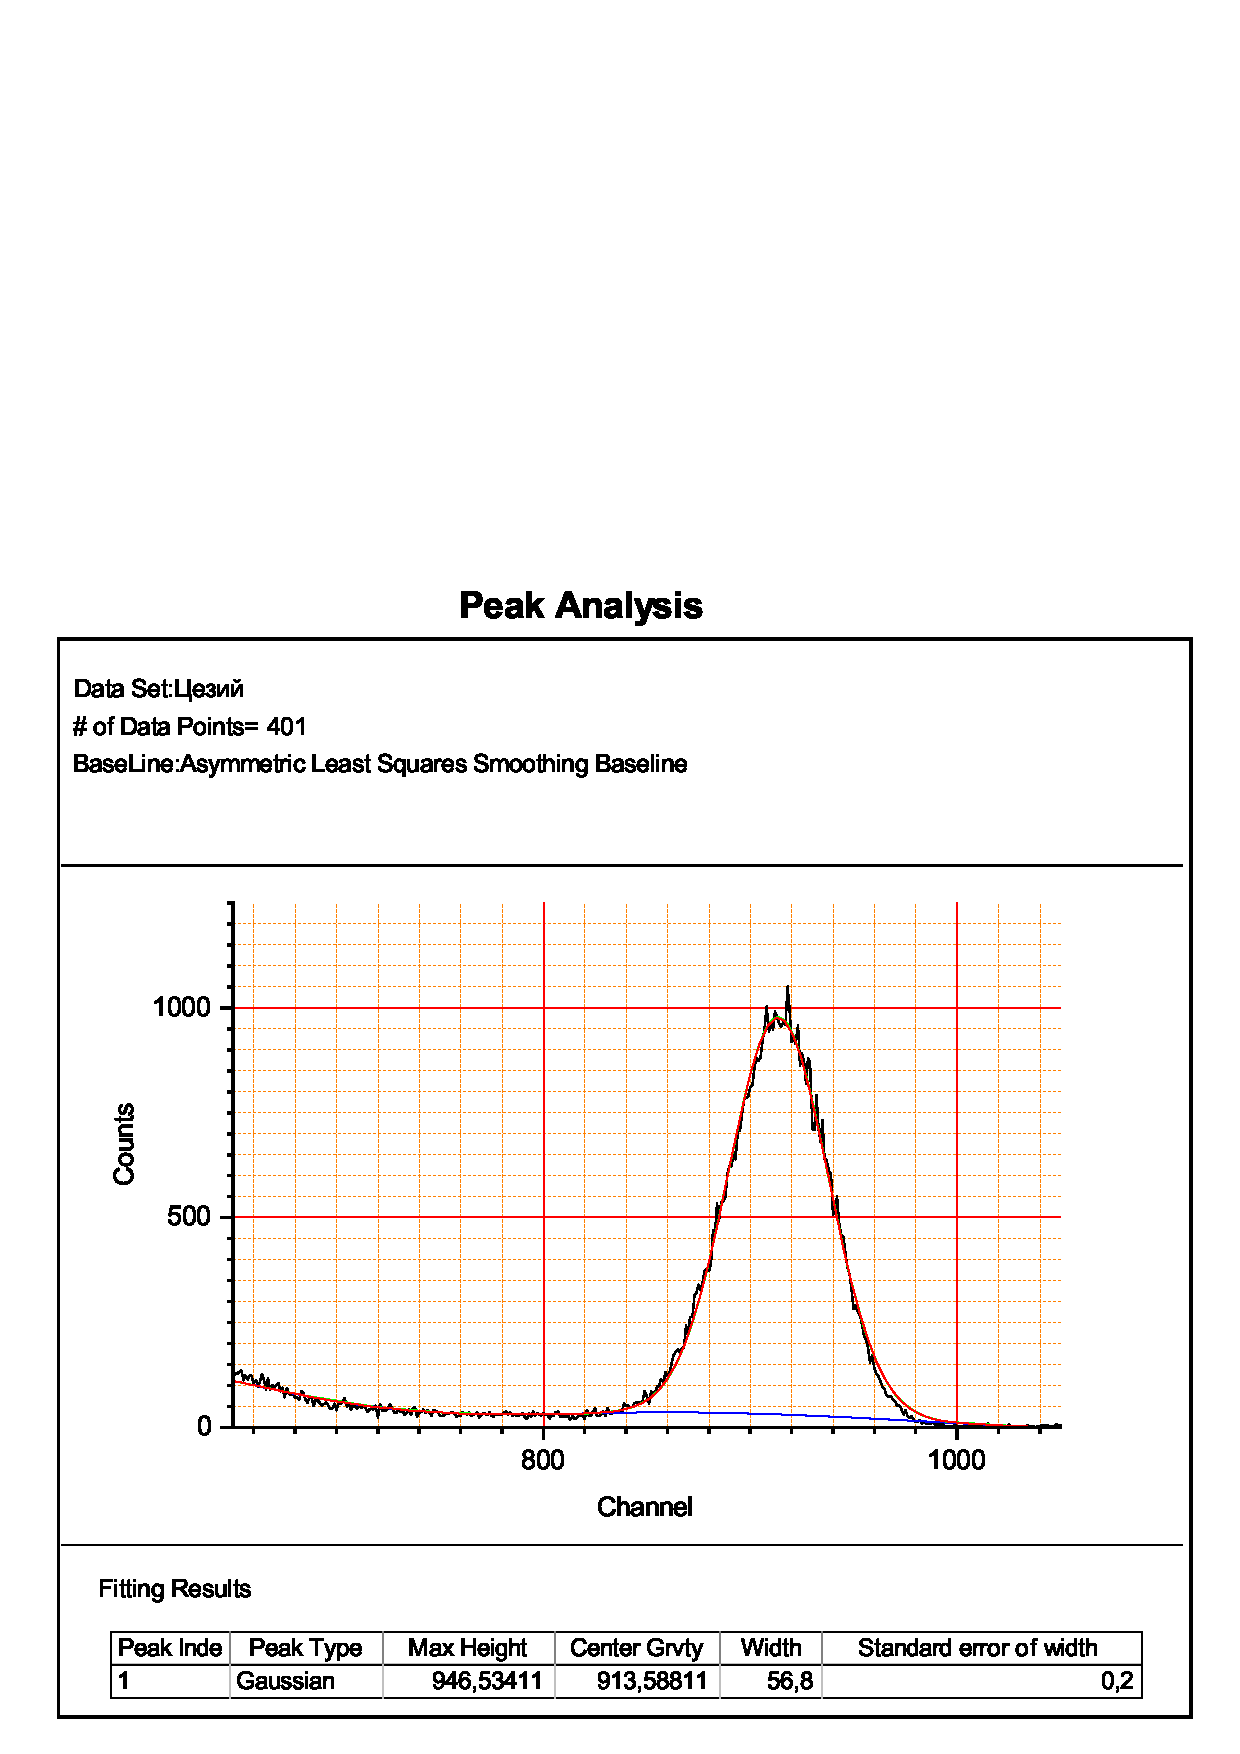
\includegraphics[width = 0.7\textwidth]{pics/3.png}
  \centering
  \caption{Схема установки 2.}
  \label{pic:setup-2}
\end{figure}
Дифракционная картина здесь наблюдается в фокальной плоскости объектива $O_2$. Каждому значению $\theta$ соответствует в этой плоскости точка, отстоящая от оптической оси на расстоянии
\begin{equation}
  X = f_2 \tan \theta \approx f_2 \theta.
\end{equation}
Объектив не вносит разности хода между интерферирующими лучам, поэтому в его фокальной плоскости наблюдается неискажённая дифракционная картина. При $\theta = 0$ разность хода между лучами нулевая, поэтому в центре поля зрения дифракционный максимум. Первый минимум соответствует $\theta_1$ такому, что в точке наблюдения разность хода пробегаем все значения от 0 до $2\pi$. Аналогично рассуждая, для $m$-й полосы
\begin{equation}
  \theta_m = \frac{m \lambda}{D}
\end{equation}
Расстояние $X_m$ тёмной полосы от оптической оси из (5) и (6)
\begin{equation}
  X_m = f_2m\frac{\lambda}{D}
\end{equation}

\subsection*{В. Дифракция Фраунгофера на двух щелях}

Для наблюдения дифракции Фраунгофера на двух щелях следует заменить щель $ S_2 $ экраном Э с двумя щелями
(рис. \ref{pic:labC}). При этом для оценки влияния ширины входной щели на чёткость дифракционной картины
вместо входной щели $ S_1 $ следует поставить щель с микрометрическим винтом. Два дифракционных изображения
входной щели, одно из которых образовано лучами, прошедшими через левую, а другое --- через правую щели,
накладываются друг на друга.

\begin{figure}[H]
  \centering
  \includegraphics[width=0.7\linewidth]{pics/setup_c.jpeg}
  \caption{Схема установки для наблюдения дифракции Фраунгофера на двух щелях}
  \label{pic:labC}
\end{figure}

Если входная щель достаточно узка, то дифракционная картина
в плоскости П (рис. \ref{pic:labC}) подобна той, что получалась при дифракции
на одной щели, однако теперь вся картина испещрена рядом дополнительных узких полос.
Угловая координата $ \theta_m $ интерференционного максимума $ m $-го порядка определяется соотношением

\begin{equation}\label{}
  \theta_m = m \dfrac{\lambda}{d}
\end{equation}

где $ d $ --- расстояние между щелями. Линейное расстояние $ \Delta x $ между соседними интерференционными полосами в плоскости П равно, поэтому

\begin{equation}\label{dx}
  \Delta x = f_2 \dfrac{\lambda}{d}
\end{equation}

На рис. \ref{pic:labC} показано распределение интенсивности в фокальной плоскости объектива $ O_2 $. Штриховой линией (в увеличенном масштабе)
изображено распределение интенсивности при дифракции света на одиночной щели. Нетрудно оценить число n интерференционных полос,
укладывающихся в области центрального дифракционного максимума.
Полная ширина главного максимума равна $ 2 f_2 \lambda /D $, где $ D $ ширина щели, отсюда

\begin{equation}\label{n}
  n = \dfrac{2f_2 \lambda}{D} \dfrac{1}{\Delta x} = \dfrac{2d}{D}
\end{equation}

При дифракции света на двух щелях чёткая система интерференционных полос наблюдается только при достаточно узкой ширине входной щели $ S $, которую можно рассматривать как протяжённый источник света размером $ b $. Для наблюдения интерференции необходимо, чтобы расстояние $ d $ между щелями не превышало радиуса когерентности

\begin{equation}\label{}
  d \ll \dfrac{\lambda}{b} f_1
\end{equation}

Здесь $ b $ --- ширина входной щели $ S $ и, следовательно, $  b/f_1 $ --- её угловая ширина. Таким образом, по размытию интерференционной картины можно оценить размер источника. Этот метод используется в звёздном интерферометре при измерении угловых размеров звёзд.

\subsection*{Г. Влияние дифракции на разрешающую способность оптического инструмента}

Установка, использованная ранее, позволяет исследовать влияние дифракции на разрешающую способность оптических инструментов.

Как уже было выяснено, линзы $O_1$ и $ O_2$ в отсутствие щели $S_2$ создают в плоскости П изображение щели $S_1$, и это изображение рассматривается в микроскоп М. Таким образом, нашу установку можно рассматривать как оптический инструмент, предназначенный для получения изображения предмета. При этом коллиматор (щель $S_1$ и объектив $O_1$) является моделью далёкого предмета, а объектив $O_2$ и микроскоп М составляют зрительную трубу, наведённую на этот предмет.
Щель $S_2$, установленная непосредственно перед объективом $O_2$, позволяет изменять эффективный размер объектива и, следовательно, разрешающую способность оптической системы.

\begin{figure}[H]
  \centering
  \includegraphics[scale=0.15]{pics/setup_d.jpeg}
  \caption{Схема установки для исследования разрешающей
    способности оптического инструмента}
  \label{pic:setup_d}
\end{figure}

Поместим вместо щели $S_1$ экран Э с двумя узкими щелями, расстояние между которыми равно $d$ (рис. \ref{pic:setup_d}). Тогда расстояние $l$ между изображениями щелей в плоскости П равно
\begin{equation}
  l = \varphi f_2 = d \dfrac{f_2}{f_1},
\end{equation}
а ширина каждого изображения
\begin{equation}
  \delta x \approx \dfrac{\lambda}{D_0} f_2
\end{equation}
определяется дифракцией света на щели $S_2$. Когда полуширина дифракционного изображения превышает расстояние между изображениями, то по виду дифракционной картины трудно определить, представляет собой источник двойную или одиночную щель.

Условия, при которых ещё можно различить, имеем мы дело с одной или двумя щелями, для разных наблюдателей различны. Для того чтобы исключить связанный с этим произвол, пользуются обычно критерием Рэлея, который приблизительно соответствует возможностям визуального наблюдения: изображения считаются различимыми, когда максимум одного дифракционного пятна совпадает с минимумом другого, а в условиях нашей задачи --- когда полуширина дифракционного изображения $\delta x$ совпадает с расстоянием $l$ между изображениями отдельных щелей:
\begin{equation}
  \delta x \sim l \to \dfrac{\lambda}{D_0} \sim \dfrac{d}{f_1}.
  \label{eq:resolution}
\end{equation}

\section{Методика измерений и результаты}
\subsection{Дифракция Френеля}

Измерим первоначальную длину щели: $ b = 0.29 \pm 0.01$ мм.
Будем приближать микроскоп к щели, по мере этого снимем зависимость координаты
микроскопа от числа $ n  $ тёмных полос по формуле $ z_n = x_n - x_0 $, где $ x_0 = 611 $
мм --- положение нуля. Результаты занесём в таб. \ref{tab:fresnel}.
В таблицу также занесём результат вычисления величины $ 2\xi_n $ по формуле (1).
При этом длина волны зелёного света $ \lambda = 5461 \cdot 10^{-10} $ м.

\begin{table}[H]
  \begin{tabular}{|c|r|r|r|r|r|r|}
    \hline
    $n$, полос & 1                 & 2                  & 3                   & 4                   & 5                  & 6                   \\ \hline
    $x_n$, см  & $ 43.4\pm0.1$     & $ 42.8\pm0.1 $     & $ 42.3\pm0.1 $      & $ 42.0 \pm 0.1 $    & $ 41.8 \pm 0.1 $   & $ 41.6 \pm 0.1 $    \\ \hline
    $z_n$, см  & $ 2.3\pm0.1 $     & $ 1.7 \pm 0.1 $    & $ 1.2 \pm 0.1 $     & $ 0.9 \pm 0.1 $     & $ 0.7 \pm 0.1 $    & $ 0.5 \pm 0.1 $     \\ \hline
    $2\xi$, мм & $0.317 \pm 0.007$ & $ 0.334 \pm 0.010$ & $ 0.324 \pm 0.013 $ & $ 0.314 \pm 0.017 $ & $0.303 \pm 0.022 $ & $ 0.277 \pm 0.028 $ \\ \hline
  \end{tabular}
  \caption{Результаты измерений для дифракции Френеля}
  \label{tab:fresnel}
\end{table}

Тогда, полагая что зоны Френеля совпадают со щелью, усредним значение ширины зон Френеля и найдем погрешность среднего:
$$h_\text{avg} = (0.311 \pm 0.004) \mim$$
$$\sqrt{\langle\sigma^2\rangle} = 0.017\mim$$
$$ h = (0.311 \pm 0.018) \mim $$

С помощью  микрометрического винта на щели найдём ширину щели
$h = (0.290 \pm 0.001) \mim$. Таким образом, наши измерения хоть и не очень точны, но все же согласуются с теорией.

\subsection{Дифракция Фраунгофера на одной щели}

С помощью нанесённой на стекло микроскопа шкалы будем измерять координаты дифракционных минимумов.
Результаты внесем в таблицу \ref{tab:fraunhofer}; построим график,рис. \ref{pic:fraunhofer}.

\begin{table}[H]
  \begin{tabular}{|l|r|r|r|r|r|r|r|r|}
    \hline
    m           & -4   & -3   & -2   & -1   & 1    & 2    & 3    & 4    \\ \hline
    $x_m, \mim$ & 1.18 & 1.34 & 1.49 & 1.65 & 2.00 & 2.17 & 2.32 & 2.48 \\ \hline
  \end{tabular}
  \caption{Результаты измерений координат для дифракции Фраунгофера}
  \label{tab:fraunhofer}
\end{table}


\begin{figure}[H]
  \includegraphics[width=0.7\linewidth]{pics/fraunhofer.png}
  \caption{Зависимость координаты минимума от его номера}
  \label{pic:fraunhofer}
\end{figure}

Введём тогда ширину между двумя минимумами $y = (0.164 \pm 0.010)\mim$, где погрешность обусловлена
приборной погрешностью (шкалы).


Учтем \textbf{фокусное расстояние линзы }$F_2 = 10~\mathrm{cm}$, тогда:
$$h = F_2 \frac{\lambda}{y} = (0.33\pm0.02)\mim,$$
при этом ширина щели по микрометру была увеличена до $(0.325\pm0.001)\mim$, что согласуется с нашим
результатом.

\subsection{Дифракция Фраунгофера на двух щелях}

Получим на экране дифракционную картину и проведём измерения и вычисления:

\begin{table}[H]
  \centering
  \caption{Измерения}
  \begin{tabular}{|c|c|c|c|} \hline
    $N$     & $X$, мм         & $\Delta x$, мкм & $d$, мм           \\
    \hline
    6$\pm$0.5 & 0.22 $\pm$ 0.01 & 36.0 $\pm$ 4.6  & 1.54 $\pm$ 0.20 \\ \hline
  \end{tabular}
\end{table}

Здесь $N$ --- число полос внутри главного максимума, $X$ --- ширина главного максимума, $\Delta x = X/n$ --- расстояние между соседними интерференционными полосами, $d = f_2 \lambda/\Delta x$ --- расстояние между щелями.

Также при помощи микроскопа измерим параметры щелей $ d $ и $ D $ <<напрямую>>. Получаем
\[ (d-D)_\text{микр} = 1.28 \pm 0.01 \text{ мм} \]
\[ D_\text{микр} = 0.28 \pm 0.01 \text{ мм} \]

Действительно, расстояние между щелями совпало с измеренным.

\subsection{Влияние дифракции на разрешающую способность оптического инструмента}
Соберём схему, заменив первую щель на экран с двойной щелью. Будем подбирать $D_0$ (рис. \ref{pic:setup-2}) такое, 
что два дфиракционных пятна становятся неразличимы. Это происходит при ширине щели в $\sim 0.120 \mim$.
Обратимся к (\ref{eq:resolution}):
$$ D_{0\text{th}} \sim \dfrac{\lambda}{d}f_1 \approx 0.60 \mim $$

Действительно, мы попали лишь в порядок. Критерий Рэлея является оценочным, и все зависит от зрения наблюдателя.


\section{Обсуждение результатов и выводы}

В ходе работы было изучено явление дифракции света - дифракция Френеля на щели и на препятствии, дифракция Фраунгофера на одной и двух щелях.

\begin{itemize}
    \item При исследовании явления дифракции Френеля на щели убедились, что ширина зон Френеля примерно равна ширине щели;
    
    \item При исследовании явления дифракции Фраунгофера на щели получили значение ширины щели, примерно равно измеренному непосредственно с помощью микрометрического винта;
    
    \item При исследовании явления дифракции Фраунгофера на двух щелях было получено значение расстояния между щелями, примерно равное измеренному с помощью микроскопа;
    
    \item При проверке критерия Рэлея сошёлся порядок минимальной ширины апертуры, при которой два объекта остаются различимыми.
    
\end{itemize}
\end{document}
